\documentclass{article} % For LaTeX2e
\usepackage{iclr2019_conference,times}

% Optional math commands from https://github.com/goodfeli/dlbook_notation.
%%%%% NEW MATH DEFINITIONS %%%%%

\usepackage{amsmath,amsfonts,bm}

% Mark sections of captions for referring to divisions of figures
\newcommand{\figleft}{{\em (Left)}}
\newcommand{\figcenter}{{\em (Center)}}
\newcommand{\figright}{{\em (Right)}}
\newcommand{\figtop}{{\em (Top)}}
\newcommand{\figbottom}{{\em (Bottom)}}
\newcommand{\captiona}{{\em (a)}}
\newcommand{\captionb}{{\em (b)}}
\newcommand{\captionc}{{\em (c)}}
\newcommand{\captiond}{{\em (d)}}

% Highlight a newly defined term
\newcommand{\newterm}[1]{{\bf #1}}


% Figure reference, lower-case.
\def\figref#1{figure~\ref{#1}}
% Figure reference, capital. For start of sentence
\def\Figref#1{Figure~\ref{#1}}
\def\twofigref#1#2{figures \ref{#1} and \ref{#2}}
\def\quadfigref#1#2#3#4{figures \ref{#1}, \ref{#2}, \ref{#3} and \ref{#4}}
% Section reference, lower-case.
\def\secref#1{section~\ref{#1}}
% Section reference, capital.
\def\Secref#1{Section~\ref{#1}}
% Reference to two sections.
\def\twosecrefs#1#2{sections \ref{#1} and \ref{#2}}
% Reference to three sections.
\def\secrefs#1#2#3{sections \ref{#1}, \ref{#2} and \ref{#3}}
% Reference to an equation, lower-case.
\def\eqref#1{equation~\ref{#1}}
% Reference to an equation, upper case
\def\Eqref#1{Equation~\ref{#1}}
% A raw reference to an equation---avoid using if possible
\def\plaineqref#1{\ref{#1}}
% Reference to a chapter, lower-case.
\def\chapref#1{chapter~\ref{#1}}
% Reference to an equation, upper case.
\def\Chapref#1{Chapter~\ref{#1}}
% Reference to a range of chapters
\def\rangechapref#1#2{chapters\ref{#1}--\ref{#2}}
% Reference to an algorithm, lower-case.
\def\algref#1{algorithm~\ref{#1}}
% Reference to an algorithm, upper case.
\def\Algref#1{Algorithm~\ref{#1}}
\def\twoalgref#1#2{algorithms \ref{#1} and \ref{#2}}
\def\Twoalgref#1#2{Algorithms \ref{#1} and \ref{#2}}
% Reference to a part, lower case
\def\partref#1{part~\ref{#1}}
% Reference to a part, upper case
\def\Partref#1{Part~\ref{#1}}
\def\twopartref#1#2{parts \ref{#1} and \ref{#2}}

\def\ceil#1{\lceil #1 \rceil}
\def\floor#1{\lfloor #1 \rfloor}
\def\1{\bm{1}}
\newcommand{\train}{\mathcal{D}}
\newcommand{\valid}{\mathcal{D_{\mathrm{valid}}}}
\newcommand{\test}{\mathcal{D_{\mathrm{test}}}}

\def\eps{{\epsilon}}


% Random variables
\def\reta{{\textnormal{$\eta$}}}
\def\ra{{\textnormal{a}}}
\def\rb{{\textnormal{b}}}
\def\rc{{\textnormal{c}}}
\def\rd{{\textnormal{d}}}
\def\re{{\textnormal{e}}}
\def\rf{{\textnormal{f}}}
\def\rg{{\textnormal{g}}}
\def\rh{{\textnormal{h}}}
\def\ri{{\textnormal{i}}}
\def\rj{{\textnormal{j}}}
\def\rk{{\textnormal{k}}}
\def\rl{{\textnormal{l}}}
% rm is already a command, just don't name any random variables m
\def\rn{{\textnormal{n}}}
\def\ro{{\textnormal{o}}}
\def\rp{{\textnormal{p}}}
\def\rq{{\textnormal{q}}}
\def\rr{{\textnormal{r}}}
\def\rs{{\textnormal{s}}}
\def\rt{{\textnormal{t}}}
\def\ru{{\textnormal{u}}}
\def\rv{{\textnormal{v}}}
\def\rw{{\textnormal{w}}}
\def\rx{{\textnormal{x}}}
\def\ry{{\textnormal{y}}}
\def\rz{{\textnormal{z}}}

% Random vectors
\def\rvepsilon{{\mathbf{\epsilon}}}
\def\rvtheta{{\mathbf{\theta}}}
\def\rva{{\mathbf{a}}}
\def\rvb{{\mathbf{b}}}
\def\rvc{{\mathbf{c}}}
\def\rvd{{\mathbf{d}}}
\def\rve{{\mathbf{e}}}
\def\rvf{{\mathbf{f}}}
\def\rvg{{\mathbf{g}}}
\def\rvh{{\mathbf{h}}}
\def\rvu{{\mathbf{i}}}
\def\rvj{{\mathbf{j}}}
\def\rvk{{\mathbf{k}}}
\def\rvl{{\mathbf{l}}}
\def\rvm{{\mathbf{m}}}
\def\rvn{{\mathbf{n}}}
\def\rvo{{\mathbf{o}}}
\def\rvp{{\mathbf{p}}}
\def\rvq{{\mathbf{q}}}
\def\rvr{{\mathbf{r}}}
\def\rvs{{\mathbf{s}}}
\def\rvt{{\mathbf{t}}}
\def\rvu{{\mathbf{u}}}
\def\rvv{{\mathbf{v}}}
\def\rvw{{\mathbf{w}}}
\def\rvx{{\mathbf{x}}}
\def\rvy{{\mathbf{y}}}
\def\rvz{{\mathbf{z}}}

% Elements of random vectors
\def\erva{{\textnormal{a}}}
\def\ervb{{\textnormal{b}}}
\def\ervc{{\textnormal{c}}}
\def\ervd{{\textnormal{d}}}
\def\erve{{\textnormal{e}}}
\def\ervf{{\textnormal{f}}}
\def\ervg{{\textnormal{g}}}
\def\ervh{{\textnormal{h}}}
\def\ervi{{\textnormal{i}}}
\def\ervj{{\textnormal{j}}}
\def\ervk{{\textnormal{k}}}
\def\ervl{{\textnormal{l}}}
\def\ervm{{\textnormal{m}}}
\def\ervn{{\textnormal{n}}}
\def\ervo{{\textnormal{o}}}
\def\ervp{{\textnormal{p}}}
\def\ervq{{\textnormal{q}}}
\def\ervr{{\textnormal{r}}}
\def\ervs{{\textnormal{s}}}
\def\ervt{{\textnormal{t}}}
\def\ervu{{\textnormal{u}}}
\def\ervv{{\textnormal{v}}}
\def\ervw{{\textnormal{w}}}
\def\ervx{{\textnormal{x}}}
\def\ervy{{\textnormal{y}}}
\def\ervz{{\textnormal{z}}}

% Random matrices
\def\rmA{{\mathbf{A}}}
\def\rmB{{\mathbf{B}}}
\def\rmC{{\mathbf{C}}}
\def\rmD{{\mathbf{D}}}
\def\rmE{{\mathbf{E}}}
\def\rmF{{\mathbf{F}}}
\def\rmG{{\mathbf{G}}}
\def\rmH{{\mathbf{H}}}
\def\rmI{{\mathbf{I}}}
\def\rmJ{{\mathbf{J}}}
\def\rmK{{\mathbf{K}}}
\def\rmL{{\mathbf{L}}}
\def\rmM{{\mathbf{M}}}
\def\rmN{{\mathbf{N}}}
\def\rmO{{\mathbf{O}}}
\def\rmP{{\mathbf{P}}}
\def\rmQ{{\mathbf{Q}}}
\def\rmR{{\mathbf{R}}}
\def\rmS{{\mathbf{S}}}
\def\rmT{{\mathbf{T}}}
\def\rmU{{\mathbf{U}}}
\def\rmV{{\mathbf{V}}}
\def\rmW{{\mathbf{W}}}
\def\rmX{{\mathbf{X}}}
\def\rmY{{\mathbf{Y}}}
\def\rmZ{{\mathbf{Z}}}

% Elements of random matrices
\def\ermA{{\textnormal{A}}}
\def\ermB{{\textnormal{B}}}
\def\ermC{{\textnormal{C}}}
\def\ermD{{\textnormal{D}}}
\def\ermE{{\textnormal{E}}}
\def\ermF{{\textnormal{F}}}
\def\ermG{{\textnormal{G}}}
\def\ermH{{\textnormal{H}}}
\def\ermI{{\textnormal{I}}}
\def\ermJ{{\textnormal{J}}}
\def\ermK{{\textnormal{K}}}
\def\ermL{{\textnormal{L}}}
\def\ermM{{\textnormal{M}}}
\def\ermN{{\textnormal{N}}}
\def\ermO{{\textnormal{O}}}
\def\ermP{{\textnormal{P}}}
\def\ermQ{{\textnormal{Q}}}
\def\ermR{{\textnormal{R}}}
\def\ermS{{\textnormal{S}}}
\def\ermT{{\textnormal{T}}}
\def\ermU{{\textnormal{U}}}
\def\ermV{{\textnormal{V}}}
\def\ermW{{\textnormal{W}}}
\def\ermX{{\textnormal{X}}}
\def\ermY{{\textnormal{Y}}}
\def\ermZ{{\textnormal{Z}}}

% Vectors
\def\vzero{{\bm{0}}}
\def\vone{{\bm{1}}}
\def\vmu{{\bm{\mu}}}
\def\vtheta{{\bm{\theta}}}
\def\va{{\bm{a}}}
\def\vb{{\bm{b}}}
\def\vc{{\bm{c}}}
\def\vd{{\bm{d}}}
\def\ve{{\bm{e}}}
\def\vf{{\bm{f}}}
\def\vg{{\bm{g}}}
\def\vh{{\bm{h}}}
\def\vi{{\bm{i}}}
\def\vj{{\bm{j}}}
\def\vk{{\bm{k}}}
\def\vl{{\bm{l}}}
\def\vm{{\bm{m}}}
\def\vn{{\bm{n}}}
\def\vo{{\bm{o}}}
\def\vp{{\bm{p}}}
\def\vq{{\bm{q}}}
\def\vr{{\bm{r}}}
\def\vs{{\bm{s}}}
\def\vt{{\bm{t}}}
\def\vu{{\bm{u}}}
\def\vv{{\bm{v}}}
\def\vw{{\bm{w}}}
\def\vx{{\bm{x}}}
\def\vy{{\bm{y}}}
\def\vz{{\bm{z}}}

% Elements of vectors
\def\evalpha{{\alpha}}
\def\evbeta{{\beta}}
\def\evepsilon{{\epsilon}}
\def\evlambda{{\lambda}}
\def\evomega{{\omega}}
\def\evmu{{\mu}}
\def\evpsi{{\psi}}
\def\evsigma{{\sigma}}
\def\evtheta{{\theta}}
\def\eva{{a}}
\def\evb{{b}}
\def\evc{{c}}
\def\evd{{d}}
\def\eve{{e}}
\def\evf{{f}}
\def\evg{{g}}
\def\evh{{h}}
\def\evi{{i}}
\def\evj{{j}}
\def\evk{{k}}
\def\evl{{l}}
\def\evm{{m}}
\def\evn{{n}}
\def\evo{{o}}
\def\evp{{p}}
\def\evq{{q}}
\def\evr{{r}}
\def\evs{{s}}
\def\evt{{t}}
\def\evu{{u}}
\def\evv{{v}}
\def\evw{{w}}
\def\evx{{x}}
\def\evy{{y}}
\def\evz{{z}}

% Matrix
\def\mA{{\bm{A}}}
\def\mB{{\bm{B}}}
\def\mC{{\bm{C}}}
\def\mD{{\bm{D}}}
\def\mE{{\bm{E}}}
\def\mF{{\bm{F}}}
\def\mG{{\bm{G}}}
\def\mH{{\bm{H}}}
\def\mI{{\bm{I}}}
\def\mJ{{\bm{J}}}
\def\mK{{\bm{K}}}
\def\mL{{\bm{L}}}
\def\mM{{\bm{M}}}
\def\mN{{\bm{N}}}
\def\mO{{\bm{O}}}
\def\mP{{\bm{P}}}
\def\mQ{{\bm{Q}}}
\def\mR{{\bm{R}}}
\def\mS{{\bm{S}}}
\def\mT{{\bm{T}}}
\def\mU{{\bm{U}}}
\def\mV{{\bm{V}}}
\def\mW{{\bm{W}}}
\def\mX{{\bm{X}}}
\def\mY{{\bm{Y}}}
\def\mZ{{\bm{Z}}}
\def\mBeta{{\bm{\beta}}}
\def\mPhi{{\bm{\Phi}}}
\def\mLambda{{\bm{\Lambda}}}
\def\mSigma{{\bm{\Sigma}}}

% Tensor
\DeclareMathAlphabet{\mathsfit}{\encodingdefault}{\sfdefault}{m}{sl}
\SetMathAlphabet{\mathsfit}{bold}{\encodingdefault}{\sfdefault}{bx}{n}
\newcommand{\tens}[1]{\bm{\mathsfit{#1}}}
\def\tA{{\tens{A}}}
\def\tB{{\tens{B}}}
\def\tC{{\tens{C}}}
\def\tD{{\tens{D}}}
\def\tE{{\tens{E}}}
\def\tF{{\tens{F}}}
\def\tG{{\tens{G}}}
\def\tH{{\tens{H}}}
\def\tI{{\tens{I}}}
\def\tJ{{\tens{J}}}
\def\tK{{\tens{K}}}
\def\tL{{\tens{L}}}
\def\tM{{\tens{M}}}
\def\tN{{\tens{N}}}
\def\tO{{\tens{O}}}
\def\tP{{\tens{P}}}
\def\tQ{{\tens{Q}}}
\def\tR{{\tens{R}}}
\def\tS{{\tens{S}}}
\def\tT{{\tens{T}}}
\def\tU{{\tens{U}}}
\def\tV{{\tens{V}}}
\def\tW{{\tens{W}}}
\def\tX{{\tens{X}}}
\def\tY{{\tens{Y}}}
\def\tZ{{\tens{Z}}}


% Graph
\def\gA{{\mathcal{A}}}
\def\gB{{\mathcal{B}}}
\def\gC{{\mathcal{C}}}
\def\gD{{\mathcal{D}}}
\def\gE{{\mathcal{E}}}
\def\gF{{\mathcal{F}}}
\def\gG{{\mathcal{G}}}
\def\gH{{\mathcal{H}}}
\def\gI{{\mathcal{I}}}
\def\gJ{{\mathcal{J}}}
\def\gK{{\mathcal{K}}}
\def\gL{{\mathcal{L}}}
\def\gM{{\mathcal{M}}}
\def\gN{{\mathcal{N}}}
\def\gO{{\mathcal{O}}}
\def\gP{{\mathcal{P}}}
\def\gQ{{\mathcal{Q}}}
\def\gR{{\mathcal{R}}}
\def\gS{{\mathcal{S}}}
\def\gT{{\mathcal{T}}}
\def\gU{{\mathcal{U}}}
\def\gV{{\mathcal{V}}}
\def\gW{{\mathcal{W}}}
\def\gX{{\mathcal{X}}}
\def\gY{{\mathcal{Y}}}
\def\gZ{{\mathcal{Z}}}

% Sets
\def\sA{{\mathbb{A}}}
\def\sB{{\mathbb{B}}}
\def\sC{{\mathbb{C}}}
\def\sD{{\mathbb{D}}}
% Don't use a set called E, because this would be the same as our symbol
% for expectation.
\def\sF{{\mathbb{F}}}
\def\sG{{\mathbb{G}}}
\def\sH{{\mathbb{H}}}
\def\sI{{\mathbb{I}}}
\def\sJ{{\mathbb{J}}}
\def\sK{{\mathbb{K}}}
\def\sL{{\mathbb{L}}}
\def\sM{{\mathbb{M}}}
\def\sN{{\mathbb{N}}}
\def\sO{{\mathbb{O}}}
\def\sP{{\mathbb{P}}}
\def\sQ{{\mathbb{Q}}}
\def\sR{{\mathbb{R}}}
\def\sS{{\mathbb{S}}}
\def\sT{{\mathbb{T}}}
\def\sU{{\mathbb{U}}}
\def\sV{{\mathbb{V}}}
\def\sW{{\mathbb{W}}}
\def\sX{{\mathbb{X}}}
\def\sY{{\mathbb{Y}}}
\def\sZ{{\mathbb{Z}}}

% Entries of a matrix
\def\emLambda{{\Lambda}}
\def\emA{{A}}
\def\emB{{B}}
\def\emC{{C}}
\def\emD{{D}}
\def\emE{{E}}
\def\emF{{F}}
\def\emG{{G}}
\def\emH{{H}}
\def\emI{{I}}
\def\emJ{{J}}
\def\emK{{K}}
\def\emL{{L}}
\def\emM{{M}}
\def\emN{{N}}
\def\emO{{O}}
\def\emP{{P}}
\def\emQ{{Q}}
\def\emR{{R}}
\def\emS{{S}}
\def\emT{{T}}
\def\emU{{U}}
\def\emV{{V}}
\def\emW{{W}}
\def\emX{{X}}
\def\emY{{Y}}
\def\emZ{{Z}}
\def\emSigma{{\Sigma}}

% entries of a tensor
% Same font as tensor, without \bm wrapper
\newcommand{\etens}[1]{\mathsfit{#1}}
\def\etLambda{{\etens{\Lambda}}}
\def\etA{{\etens{A}}}
\def\etB{{\etens{B}}}
\def\etC{{\etens{C}}}
\def\etD{{\etens{D}}}
\def\etE{{\etens{E}}}
\def\etF{{\etens{F}}}
\def\etG{{\etens{G}}}
\def\etH{{\etens{H}}}
\def\etI{{\etens{I}}}
\def\etJ{{\etens{J}}}
\def\etK{{\etens{K}}}
\def\etL{{\etens{L}}}
\def\etM{{\etens{M}}}
\def\etN{{\etens{N}}}
\def\etO{{\etens{O}}}
\def\etP{{\etens{P}}}
\def\etQ{{\etens{Q}}}
\def\etR{{\etens{R}}}
\def\etS{{\etens{S}}}
\def\etT{{\etens{T}}}
\def\etU{{\etens{U}}}
\def\etV{{\etens{V}}}
\def\etW{{\etens{W}}}
\def\etX{{\etens{X}}}
\def\etY{{\etens{Y}}}
\def\etZ{{\etens{Z}}}

% The true underlying data generating distribution
\newcommand{\pdata}{p_{\rm{data}}}
% The empirical distribution defined by the training set
\newcommand{\ptrain}{\hat{p}_{\rm{data}}}
\newcommand{\Ptrain}{\hat{P}_{\rm{data}}}
% The model distribution
\newcommand{\pmodel}{p_{\rm{model}}}
\newcommand{\Pmodel}{P_{\rm{model}}}
\newcommand{\ptildemodel}{\tilde{p}_{\rm{model}}}
% Stochastic autoencoder distributions
\newcommand{\pencode}{p_{\rm{encoder}}}
\newcommand{\pdecode}{p_{\rm{decoder}}}
\newcommand{\precons}{p_{\rm{reconstruct}}}

\newcommand{\laplace}{\mathrm{Laplace}} % Laplace distribution

\newcommand{\E}{\mathbb{E}}
\newcommand{\Ls}{\mathcal{L}}
\newcommand{\R}{\mathbb{R}}
\newcommand{\emp}{\tilde{p}}
\newcommand{\lr}{\alpha}
\newcommand{\reg}{\lambda}
\newcommand{\rect}{\mathrm{rectifier}}
\newcommand{\softmax}{\mathrm{softmax}}
\newcommand{\sigmoid}{\sigma}
\newcommand{\softplus}{\zeta}
\newcommand{\KL}{D_{\mathrm{KL}}}
\newcommand{\Var}{\mathrm{Var}}
\newcommand{\standarderror}{\mathrm{SE}}
\newcommand{\Cov}{\mathrm{Cov}}
% Wolfram Mathworld says $L^2$ is for function spaces and $\ell^2$ is for vectors
% But then they seem to use $L^2$ for vectors throughout the site, and so does
% wikipedia.
\newcommand{\normlzero}{L^0}
\newcommand{\normlone}{L^1}
\newcommand{\normltwo}{L^2}
\newcommand{\normlp}{L^p}
\newcommand{\normmax}{L^\infty}

\newcommand{\parents}{Pa} % See usage in notation.tex. Chosen to match Daphne's book.

\DeclareMathOperator*{\argmax}{arg\,max}
\DeclareMathOperator*{\argmin}{arg\,min}

\DeclareMathOperator{\sign}{sign}
\DeclareMathOperator{\Tr}{Tr}
\let\ab\allowbreak

\usepackage{todonotes}
\usepackage{hyperref}
\usepackage{url}
\usepackage{algorithm}
\usepackage{algorithmic}
\usepackage{amsthm,amssymb}
\usepackage[utf8]{inputenc}
\newtheorem{theorem}{Theorem}
\newtheorem{lemma}{Lemma}
\graphicspath{{figures/}}
% \usepackage[pdftex]{graphicx}


\title{On the connection between stochastic optimization and splitting scheme for ODE.}

% Authors must not appear in the submitted version. They should be hidden
% as long as the \iclrfinalcopy macro remains commented out below.
% Non-anonymous submissions will be rejected without review.

\author{Daniil Merkulov \& Ivan Oseledets \\
Skolkovo Institute of Science and Technology\\
Center for Computational and Data-Intensive Science and Engineering\\
Bolshoy Boulevard 30, bld. 1, Moscow, Russia 121205 \\
\texttt{\{daniil.merkulov, i.oseledets\}@skoltech.ru} \\
}

% The \author macro works with any number of authors. There are two commands
% used to separate the names and addresses of multiple authors: \And and \AND.
%
% Using \And between authors leaves it to \LaTeX{} to determine where to break
% the lines. Using \AND forces a linebreak at that point. So, if \LaTeX{}
% puts 3 of 4 authors names on the first line, and the last on the second
% line, try using \AND instead of \And before the third author name.

\newcommand{\fix}{\marginpar{FIX}}
\newcommand{\new}{\marginpar{NEW}}

\iclrfinalcopy % Uncomment for camera-ready version, but NOT for submission.
\begin{document}


\maketitle

\begin{abstract}
We present different view on stochastic optimization, which goes back to the splitting schemes for approximate solutions of ODE. In this work we provide a connection between stochastic gradient descent approach and first order splitting scheme for ODE. We present, that the Kaczmarz method is the limit case of the splitting scheme for unitary batch SGD linear least squares approach. We support our findings with empirical tests.
\end{abstract}

\tableofcontents

%================================================
% Introduction
%================================================

\section{Introduction}
A lot of practical problems arising in machine learning require minimization of a finite sample average which can be written in the form
\begin{equation}\label{strang:finitesum}
    f(\theta) = \frac{1}{n} \sum_{i=1}^n f_i(\theta) \rightarrow \min_{\theta \in \mathbb{R}^p},
\end{equation}
where the sum goes over the \emph{minibatches} of the original dataset. Vanilla stochastic gradient descent (SGD) method (\cite{robbins1951stochastic})has consists in sequential step in the direction of the gradient of $f_i(\theta)$, where $i$ is to be chosen randomly from $1$ to $n$ without replacement.
$$
\theta_{k+1} = \theta_{k} - h_{k} \nabla f_i.
$$
Gradient descent method can be considered as an Euler discretization of the ordinary differential equation (ODE) of the form of the gradient flow
\begin{equation}\label{strang:euler}
    \frac{d \theta}{d t} = -\nabla f(\theta).
\end{equation}
In continuous time, SGD if often analyzed by introducing a noise into the right-hand side of \eqref{strang:euler}. However, for real dataset the distribution of the noise obtained by replacing the full gradient by its minibatch variant is not known and can be different for different problems. Instead, we propose a new view on the SGD as a \emph{first-order splitting scheme} for \eqref{strang:euler}, thus shedding a new light on SGD-type algorithms. This representation allows to use more efficient splitting schemes for the approximation of the full gradient flow. We show, that second-order Marchuk/Strang splitting scheme (\cite{marchuk1968some}, \cite{strang1968construction}) provides faster convergence 

% We'll leave SAG for a moment.. Moreover, we interpret stochastic average gradient (SAG)\cite{schmidt2017minimizing} approach as the \emph{splitting scheme with rebalancing} of the SAG method, which we call \emph{SAG2} method. In implementation, the second-order scheme consists in a sequential processing of minibatches first from $1$ to $m$, and then from $m$ to $1$, i.e. a single iteration of SAG2 has the same cost as two iterations of SAG.

\textbf{Contributions}
\begin{itemize}
    \item We show, that vanilla SGD could be considered as a splitting scheme for a full gradient flow.
    \item We demonstrate the connection between rebalancing splitting and stochastic average gradient method.
    \item We propose new optimization method, SAG2 based on second order splitting scheme and show that it gives better convergence, than the standard SAG method.
    % Перспективные вещи - аналитическая связь размера батча и величины шага, устойчивость к шагу
\end{itemize}

%================================================
% SGD as a splitting scheme
%================================================

\section{SGD as a splitting scheme}

We want to establish the connection between splitting scheme for ODE and stochastic optimization. In this section we firstly consider simple ODE, where we can apply splitting idea and corresponding minimization problem.

\subsection{Splitting schemes for ODEs}
The best example to start from is simple ODE with right-hand-side, consisting of two summands:
\begin{equation}
    \dfrac{d \theta}{d t} = - \frac{1}{2} \left( g_1(\theta) + g_2(\theta)\right)
    \label{strang:gradientflow}
\end{equation}
Suppose, we want to find the solution $\theta(h)$ of \eqref{strang:gradientflow} via integrating it on the small timestep $h$. The first order splitting scheme defined by solving first:
$$
\dfrac{d \theta}{d t} = - \frac{1}{2} g_1(\theta)
$$
with exact solution $\theta_1(h)$ at the moment $h$ , followed by
$$
\dfrac{d \theta}{d t} = - \frac{1}{2} g_2(\theta)
$$
with exact solution $\theta_2(h)$ at the moment $h$. Thus, the first order approximation could be written as a combinations of both solutions:
$$
\theta^I(h) = \theta_2(h) \circ \theta_1(h) \circ \theta_0,
$$
while the second order scheme takes 3 substeps:
$$
\theta^{II}(h) = \theta_1\left(\frac{h}{2}\right) \circ \theta_2(h) \circ \theta_1\left(\frac{h}{2}\right) \circ \theta_0
$$
Order of scheme defines the degree of polynomial of $h$, up to which the true solution and approximation are coincide. The local error of both schemes could be obtained by Baker - Campbell - Hausdorff formula (\cite{baker1901further}, \cite{campbell1896law}, \cite{hausdorff1906symbolische})
\begin{equation}
    \label{strang:lie_error}
    \theta^I(h) - \theta(h) = \dfrac{h^2}{2} \left[g_{1}, g_{2}\right] \theta_0 + o(h^3),
\end{equation}
\begin{equation}
    \label{strang:marchuk_error}
    \theta^{II}(h) - \theta(h) = h^{3} \left(\frac{1}{12}[g_2,[g_2, g_1]]-\frac{1}{24}[g_1,[g_1, g_2]]\right)\theta_0+O\left(h^{4}\right)
\end{equation}

where $\left[ g_1, g_2\right] = \dfrac{d g_1}{d \theta} g_2 - \dfrac{d g_2}{d \theta} g_1 $ stands for commutator of the vector fields $g_1$ and $g_2$. The $\theta_0 = \theta(0)$ for initial condition of original ODE.

Note, that the basic idea of splitting could be also applied, when the number of terms in the right-hand side of ODE is greater, than two. In this case splitting scheme will take the following form:
\begin{equation}\label{strang:marchuk}
	\theta^I(h) = \theta_m(h) \circ \theta_{m-1} \circ \ldots \circ \theta_2(h) \circ \theta_1(h) \circ \theta_0
\end{equation}
\begin{equation}\label{strang:strang}
	\theta^{II}(h) = \theta_1\left(\frac{h}{2}\right) \circ \theta_2\left(\frac{h}{2}\right) \circ\ldots \theta_m(h) \ldots \theta_2\left(\frac{h}{2}\right) \circ \theta_1\left(\frac{h}{2}\right) \circ \theta_0
\end{equation}

\subsection{SGD as approximation for the Gradient Flow equation}
Now we consider classical SGD method as a splitting scheme for the full gradient descent (\cite{cauchy1847methode}). Suppose, we have the simplest ($m=2$) finite sum minimization problem:
$$
\min_{\theta \in \sR^n} \dfrac{1}{m}\sum\limits_{i=1}^m f_i(\theta) = \min_{\theta \in \sR^n} \frac{1}{2} \left( f_1(\theta) + f_2(\theta)\right)
$$
Let us denote by $g_i^k = \nabla f_i(\theta_k)$, than, the vanilla gradient descent will be written as
$$
\theta_{k+1} = \theta_k - h\cdot\frac{1}{2} \left( g^k_1(\theta) + g^k_2(\theta)\right),
$$
while SGD version will take steps iteratively over minibatch gradient directions:
\begin{align*}\label{strang:sgd2}
\theta_{k+1} &= \theta_k - h\cdot g^k_1(\theta) \\
\theta_{k+2} &= \theta_{k+1} - h\cdot  g^{k+1}_2(\theta)
\end{align*}
These two iterations forms an epoch in SGD approach. Each of the substeps can be considered as a forward Euler method for the discretization of the ODE for a timestep $h$
\begin{align*}
    \frac{d \theta^I}{d t} = -g_1(\theta), \quad \theta^I(0) = \theta_{k},\\
    \frac{d \theta^{II}}{d t} = -g_2(\theta), \quad \theta^{II}(0) = \theta^{I}(h),
\end{align*}
therefore the final result for a sufficiently small $h$ approximates the gradient flow for at time $t + h$. The vanilla gradient descent, however, is only approximating the gradient flow at time $t + h/2$. For larger number of minibatches, rather then the GD flow. One can notice, that in SGD we use a very simple time integration inside the substep. In some cases, we can integrate the subproblem exactly, without using forward Euler scheme. Generalized linear models are among such problems, but we will first study the linear least squares case in more details, since in this case we can obtain non-trivial error bounds.

\subsection{Splitting approximation for the Gradient Flow equation}

It is interesting to look how the pure splitting scheme corresponds to the SGD approach. For this purpose we consider illustrative example of Gradient Flow equation \ref{strang:simple_GF}, where the right-hand side of ODE is just the sum of operators acting on $\theta$, which allows us to apply splitting scheme approximation directly.
\begin{equation}
\label{strang:simple_GF}
\dfrac{d \theta}{d t} = -\dfrac{1}{2} \sum\limits_{i=1}^2 \nabla f_i (\theta) = - \dfrac{1}{2} \nabla f_1 (\theta) -\dfrac{1}{2}  \nabla f_2 (\theta)
\end{equation}

In order to establish the connection between splitting scheme and SGD we use the Euler discretization below:

\begin{align*}
% \label{strang:simple_GF_splitting}
&\text{First splitting step: } &\dfrac{d \theta}{d t} = -\frac{1}{2}\nabla f_1(\theta)  &\to\text{ Euler discretization}\to &\tilde{\theta}_{I} = \theta_0 - \frac{h}{2}\nabla f_1 (\theta_0) \\
&\text{Second splitting step: } &\dfrac{d \theta}{d t} = -\frac{1}{2}\nabla f_2(\theta)  &\to\text{ Euler discretization}\to &\theta_{I} = \tilde{\theta}_{I} - \frac{h}{2}\nabla f_2 (\tilde{\theta}_{I})
\end{align*}
\begin{align*}
% \label{strang:simple_GF_splitting}
&\qquad\text{SGD epoch} &\text{First order splitting} \\
&\tilde{\theta}_{SGD} = \theta_0 - h \nabla f_1 (\theta_0) &\tilde{\theta}_{I} = \theta_0 - \frac{h}{2}\nabla f_1 (\theta_0) \\
&\theta_{SGD} = \tilde{\theta}_{SGD} - h \nabla f_2 (\tilde{\theta}_{SGD}) &\theta_{I} = \tilde{\theta}_{I} - \frac{h}{2}\nabla f_2 (\tilde{\theta}_{I})
\end{align*}

Thus, we can conclude, that \textit{one epoch of SGD is just the splitting scheme for the discretized Gradient Flow ODE with $2 \cdot h$ step size ($m \cdot h$ in case of $m$ batches)}

This idea gives additional intuition on the method. Both approaches are solving local problems through the Euler discretization. Given an information about the Euler scheme limitation, why not solve these local problems more accurate?

\subsection{Upper bound on the global splitting error}

Suppose, that we have only two batches, and the problem \eqref{strang:linearlst} is consistent, i.e. there exists an exact solution $\theta_*$ such as $X \theta_* = y$. The GD flow has the form
\begin{equation}\label{strang:model1}
    \frac{d \theta}{d t} = -X^{\top} (X \theta - y) = -X^{\top} X(\theta - \theta_*) = -(X_1^{\top} X_1 + X^{\top}_2 X_2)(\theta - \theta_*),
\end{equation}
i.e. the splitting scheme corresponds to a linear operator splitting

$$
A = A_1 + A_2, \quad A = -X^{\top} X, \quad A_i = -X^{\top}_i X_i, \quad i = 1, 2.
$$

Both $A_1$ and $A_2$ are symmetric non-negative definite matrices. Without loss of generality, we can assume that $\theta_* = 0$,

Suppose that the rank of $A$ is $r_1$ and the rank of $A_2$ is $r_2$. Then, we can write them as
$$
A_i = Q_i B_i Q^*_i,
$$
where $Q_i$ is an $N \times r_i$ matrix with orthonormal columns.  The following Lemma gives the representation of the matrix exponents of such matrices.
\begin{lemma}\label{strang:lemexp}
Let $A = Q B Q^*,$ where $Q$ is an $N \times r$ matrix with orthonormal columns, and $B$ is an $r \times r$ matrix. Then,
\begin{equation}\label{strang:lrexp}
    e^{t A}  = (I - QQ^*) + Q e^{t B} Q^*.
\end{equation}
\end{lemma}
To prove \eqref{strang:lrexp} we note that
$$e^{t A} = \sum_{k=0}^{\infty} \frac{t^k A^k}{k!} = \sum_{k=0}^{\infty} \frac{t^k Q B^k Q^*}{k!} =
I - QQ^* + QQ^* + Q \sum_{k=1}^{\infty} \frac{t^k B^k}{k!} Q^* = (I - QQ^*) + Q e^{t B} Q^*.
$$

\begin{lemma}
	\label{strang:lemupper_2}
	Let $A_1, A_2 \in \mathbb{S}^p_{+}$ be the square negative semidefinite matrices, that don't have full rank, i.e. $\operatorname{rank}{A_1} \leq p$ and $\operatorname{rank}{A_2} \leq p$. While the sum of those matrices has full rank, i.e. $A = A_1 + A_2, \operatorname{rank}{A} = p$. Then, the global upper bound error will be written as follows:

	\begin{equation}\label{strang:lemupper}
		\lim_{t \to \infty}\| e^{A_2t}e^{A_1t} - e^{At}\| = \|(I - Q_2Q_2^*)(I - Q_1Q_1^*)\|
	\end{equation}
\end{lemma}
\begin{proof}
	The proof is straightforward. We will use the low rank matrix exponential decomposition from the Lemma \ref{strang:lemexp}
	$$
	e^{A_it} = \Pi_i + Q_i e^{B_it} Q_i^*, \text{where } \Pi_i = I - Q_iQ_i^*; i = 1,2
	$$
	\begin{align*}
	\lim_{t \to \infty}\| e^{A_2t}e^{A_1t} - e^{At}\| = \lim_{t \to \infty}\| (\Pi_2 + Q_2 e^{B_2t} Q_2^*)(\Pi_1 + Q_1 e^{B_1t} Q_1^*) - e^{At}\| = \\
	= \lim_{t \to \infty}\| \Pi_2\Pi_1 + Q_1 e^{B_1t} Q_1^*\Pi_2 + \Pi_1Q_2 e^{B_2t} Q_2^* +  Q_1 e^{B_1t} Q_1^* Q_2 e^{B_2t} Q_2^* - e^{At}\| = \Pi_2 \Pi_1
	\end{align*}
	Since all matrices $B_1, B_2, A$ are negative all the matrix exponentials are decaying: $\|e^{At}\|\leq e^{t\mu (A)}\, \forall t\geq 0$, where $\mu(A) = \lambda_{max} \left( \dfrac{A + A^\top}{2}\right)$ - the logarithmic norm.
\end{proof}

\begin{figure}[h!]
	\centering
	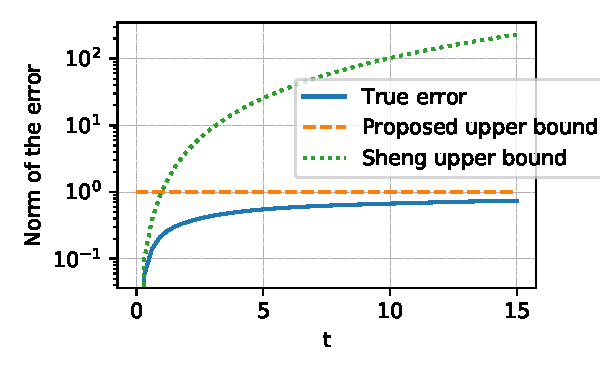
\includegraphics[width=0.6\textwidth]{upper_bound_2.pdf}
	\caption{Global error of the splitting scheme. Initial random full rank matrix $X \in \mathbb{R}^{100 \times 100}$ was splitted by rows. $X_1, X_2 \in \mathbb{R}^{50 \times 100}$. Target matrices were obtained the following way: $A_1 = -X_1^*X_1, A_2 = -X_2^*X_2, A = -X^*X$. So $A_1, A_2$ are negative and lacking full rank, while $A = A_1 + A_2$ has full rank.}
	\label{strang:fig:upper_bound_2}
\end{figure}

The graph presented on the Figure \ref{strang:fig:upper_bound_2} describes . One can easily see significant difference between existing global upper bounds for that case (\cite{sheng1994global}) and derived upper bound.

\begin{theorem}\label{strang:theorem_uppbound}
	Let $A_1, A_2, \ldots, A_b \in \mathbb{S}^p_{+}$ be the square negative semidefinite matrices, that don't have full rank, i.e. $\operatorname{rank}{A_i} \leq p, \;\forall i = 1, \ldots, b$. While the sum of those matrices has full rank, i.e. $A = \sum\limits_{i=1}^b A_i, \operatorname{rank}{A} = p$. Then, the global upper bound error will be written as follows:

	\begin{equation}\label{strang:global_error_upper_bound}
		\lim_{t \to \infty}\| e^{A_bt} \cdot \ldots \cdot e^{A_1t} - e^{At}\| = \left\|\prod\limits_{i=1}^b \Pi_{b-i+1}\right\|,
	\end{equation}
	where $\Pi_i = I - Q_iQ_i^*$ and $A_i = Q_iB_iQ_i^*$ and $Q_i$ ia a matrix with orthonormal columns. 
\end{theorem}

\begin{figure}[h!]
	\centering
	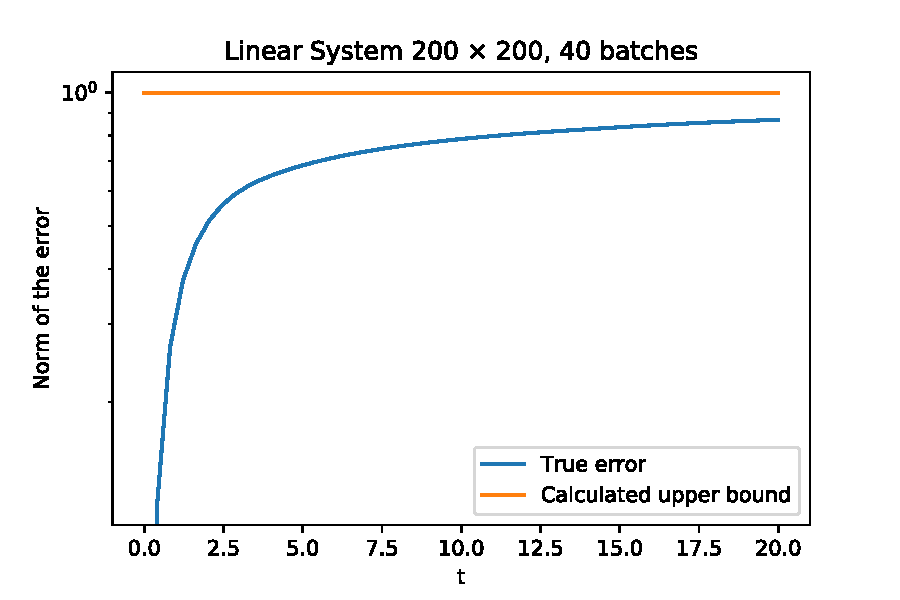
\includegraphics[width=0.6\textwidth]{upper_bound_many.pdf}
	\caption{Global upper bound on the splitting scheme in case of $40$ summands in the right-hand side. }
	\label{strang:fig:upper_bound_many}
\end{figure}

The graph on the Figure \ref{strang:fig:upper_bound_many} shows empirical validity of the presented upper bound.


%================================================
% Applications
%================================================

\section{Applications}
\subsection{Linear least squares}
\subsubsection{Problem}
Let $f_i(\theta) = \Vert x_i^{\top} \theta - y_i \Vert^2$, then problem \eqref{strang:finitesum} is the linear least squares problem, which can be written as
\begin{equation}\label{strang:LLS}
   f(\theta) = \dfrac{1}{n}\Vert X \theta - y \Vert_2^2  = \dfrac{1}{n}\sum\limits_{i=1}^s\Vert X_i \theta - y_i \Vert_2^2\to \min_{\theta \in \mathbb{R}^p},
\end{equation}
where $X$ in an $n \times p$ matrix, and $y$ is a vector of length $p$ and the second part of the equation stands for $s$ mini-batches with size $b$ regrouping ($b \cdot s = n$): $X_i \in \mathbb{R}^{b \times p}, y_i \in \mathbb{R}^{b}$

\begin{equation}\label{strang:LLS_grad}
\nabla_\theta f(\theta) = \nabla f(\theta) = \dfrac{1}{n}\sum\limits_{i=1}^s X_i^\top( X_i \theta - y_i)
\end{equation}

The gradient flow equation will be written as follows:
\begin{equation}\label{strang:LLS_GF}
\dfrac{d \theta}{d t} = - \dfrac{1}{n}\sum\limits_{i=1}^s X_i^\top( X_i \theta - y_i)
\end{equation}

\subsubsection{Exact solution of the local problem}
On each splitting approximation step we need to solve the local problem:
\begin{equation}\label{strang:LLS_local_problem}
\dfrac{d \theta}{d t} = - \dfrac{1}{n} X_i^\top( X_i \theta - y_i)
\end{equation}
\begin{theorem}\label{strang:LLS_local_solution} For any matrix $X_i \in \mathbb{R}^{b \times p}$, any vector of right-hand side $y_i \in \mathbb{R}^{b}$ and initial vector of parameters $\theta_0$, there is a solution of the ODE in \ref{strang:LLS_local_problem}, given by formula:
$$
\theta(h) = Q_i e^{-\frac{1}{n}R_iR_i^\top h} \left( Q_i^\top \theta_0 - R_i^{-\top}y_i\right) + Q_iR_i^{-\top}y_i + (I - Q_iQ_i^\top)\theta_0,
$$ 
where $Q_i \in \mathbb{R}^{p \times b}$ and $R_i \in \mathbb{R}^{b \times b}$ stands for the $QR$ decomposition of the matrix $X_i^\top$, $X_i^\top = Q_i R_i$.
\end{theorem}

\begin{proof}
Given $X_i^\top = Q_i R_i$, we have $(I - Q_iQ_i^\top)X_i^\top = 0$. Note, that $Q_i$ is left unitary matrix, i.e. $Q_i^\top Q_i = I$. 
\begin{align}
\nonumber \dfrac{d \theta}{d t} &= - \dfrac{1}{n} X_i^\top( X_i \theta - y_i) \\
\nonumber (I - Q_iQ_i^\top)\dfrac{d \theta}{d t} &= 0 \\
\nonumber \dfrac{d \theta}{d t} &= Q_i\dfrac{d (Q_i^\top\theta)}{d t} \quad Q_i^\top \theta = \eta_i\\ 
\nonumber \dfrac{d \theta}{d t} &= Q_i\dfrac{d \eta_i}{d t} \quad \text{integrate from $0$ to $h$}\\ 
\label{strang:lls_theorem_theta_from_eta}\theta(h) &= Q_i \left(\eta_i(h) - \eta_i(0) \right) + \theta_0
\end{align}

On the other hand:
\begin{align}\nonumber
\dfrac{d \eta_i}{d t} &= Q_i^\top\dfrac{d \theta}{d t} =  - \dfrac{1}{n} Q_i^\top  X_i^\top( X_i \theta - y_i) = - \dfrac{1}{n} Q_i^\top  Q_i R_i( R_i^\top Q_i^\top \theta - y_i) =\\ 
&= - \dfrac{1}{n} \left( R_iR_i^\top \eta_i - R_i y_i\right) \label{strang:lls_theorem_eta_from_theta}
\end{align}

Consider the moment of time $t = \infty$. $\dfrac{d \eta}{d t} = 0$, since $\exists \theta^*, Q_i^\top \theta^* = \eta_i^*$. Also consider \ref{strang:lls_theorem_eta_from_theta}:
\todo[inline]{Need to clarify this assumption}

\begin{equation}\label{strang:lls_theorem_eta_star}
\dfrac{d \eta_i}{d t} = 0 = - \dfrac{1}{n} \left( R_iR_i^\top \eta_i^* - R_i y_i\right) \quad \rightarrow \quad R_i y_i = R_iR_i^\top \eta_i^*
\end{equation}

Now we look at the \ref{strang:lls_theorem_eta_from_theta} with the replacement, given in \ref{strang:lls_theorem_eta_star}:

\begin{align*}
\dfrac{d \eta_i}{d t} &= - \dfrac{1}{n} \left( R_iR_i^\top \eta_i- R_iR_i^\top \eta_i^*\right) \\
\dfrac{d \eta_i}{d t} &= - \dfrac{1}{n} R_iR_i^\top \left( \eta_i- \eta_i^*\right) \qquad \text{integrate from $0$ to $h$} \\
\eta_i(h) - \eta_i^* &= e^{- \frac{1}{n} R_iR_i^\top h} (\eta_i(0) - \eta_i^*) \qquad \eta_i^* = R_i^{-\top}y_i, \eta_i(0) = Q_i^\top \theta_0 \\ 
\eta_i(h) &= e^{- \frac{1}{n} R_iR_i^\top h} (Q_i^\top \theta_0 - R_i^{-\top}y_i) + R_i^{-\top}y_i 
\end{align*}

Using \ref{strang:lls_theorem_theta_from_eta} we obtain the target formula
$$
\theta(h) = Q_i \left(e^{- \frac{1}{n} R_iR_i^\top h} (Q_i^\top \theta_0 - R_i^{-\top}y_i) + R_i^{-\top}y_i - Q_i^\top \theta_0 \right) + \theta_0
$$

\end{proof}
In case of the linear right-hand side of an ODE it is easy to solve it analytically. Now let see how the splitting approximation itself depends on the step size $h$.
$$\theta^{GD} (h) = e^{-Ah} \theta, $$
and splitting gives
$$\theta^{SGD}(h) = e^{-A_1 h} e^{-A_2 h} \theta.$$
The error is bounded as
$$
 \Vert \theta^{GD} (h) - \theta^{SGD}(h) \Vert \leq  \Vert E_1(h) \Vert \Vert \theta \Vert,
$$
where
\begin{equation}\label{strang:error}
E_1(t) = e^{A t} - e^{A_1 t} e^{A_2 t}.
\end{equation}
We need to bound the norm of the matrix $E_1(t)$ for all $h$, not only for small ones, i.e. we need global estimates. Such kind of estimates were obtained in \cite{sheng1994global} and have the form
\begin{equation}\label{strang:sheng}
    \Vert E(t) \Vert \leq \frac{t^2}{2} \Vert [ A_1, A_2] \Vert \max \{ e^{t \mu(A_1 + A_2}), e^{t(\mu(A_1) + \mu(A_2))}\},
\end{equation}
where $\mu(Z)$ is the largest eigenvalue of the matrix $\frac{Z+Z^*}{2},$ but in our case all matrices are symmetric, thus these are largest eigenvalues of the matrix. The estimate \eqref{strang:sheng} and its generalization to a larger number of summands is not very useful for us, since we will have matrices $X_i$ that have fewer rows, than column, i.e. matrices $A_i$ will have zero eigenvalues, thus the the maximum term will be equal to $1$, and the upper bound will grow quadratically with $h$. In reality, the behaviour is very different, see Figure~\ref{strang:modelfig}. In this example, we took $N=p=2$, batch size $1$. It can be seen, that the true error reaches a plateu, whereas the upper bound is growing quadratically with $t$.

We will now prove a better upper bound, that takes into account  possible zero eigenvalues of the matrices $A_1$ and $A_2$.


\subsubsection{Kaczmarz as the limit case of splitting}

\subsection{Binary logistic regression}
\subsubsection{Problem}
In this classification task then problem \eqref{strang:finitesum} takes the following form:
\begin{equation}\label{strang:LogReg}
   f(\theta) = -\dfrac{1}{n} \left(y_i \ln h_{\theta}(x_i)  + (1-y_i) \ln (1-h_{\theta}(x_i))\right) \to \min_{\theta \in \mathbb{R}^p},
\end{equation}
where $h_\theta(x_i) = \dfrac{1}{1 + e^{-\theta^\top x_i}}$ is the hypothesis function with given parameter $\theta$ from the object $x_i$, $ y_i \in \{0,1\}$ stands for the label of the object class.

\begin{equation}\label{strang:LogReg_grad}
\nabla_\theta f(\theta) = \nabla f(\theta) = \dfrac{1}{n}\sum\limits_{i=1}^n x_i(h_\theta(x_i) - y_i)
\end{equation}

The gradient flow equation will be written as follows:
\begin{equation}\label{strang:LogReg_GF}
\dfrac{d \theta}{d t} = - \dfrac{1}{n}\sum\limits_{i=1}^n x_i(h_\theta(x_i) - y_i)
\end{equation}


\subsection{Softmax regression}
\subsection{Problem}

%================================================
% Results
%============================={}===================

\section{Results}
\subsection{Iteration comparison}
\subsection{Time comparison}
\subsection{Robustness to stepsize choosing}


%================================================
% Related work
%================================================

\section{Related work}

In \cite{su2014differential} authors introduced second order ODE, which is equivalent (in the limit sense) to the gradient descent with Nesterov momentum \cite{nesterov1983method}. The paper contains both formal and intuitive derivation of the proposed ODE from the iterative method itself with analogous upper bounds for general convex optimization setting and closed form solution for quadratic function. Strongly convex and composite optimizations are also covered. Theoretical conclusions are supported by strong empirical results on the variety of test functions.



% https://na.math.kit.edu/marlis/download/talks/05helsinki_ostermann.pdf
% https://ocw.mit.edu/courses/mathematics/18-336-numerical-methods-for-partial-differential-equations-spring-2009/lecture-notes/MIT18_336S09_lec20.pdf
% https://hal.archives-ouvertes.fr/hal-01183745/document


%================================================
% Appendix
%================================================

\appendix
\section{Proofs}
\section{Additional graphs}


\begin{figure}
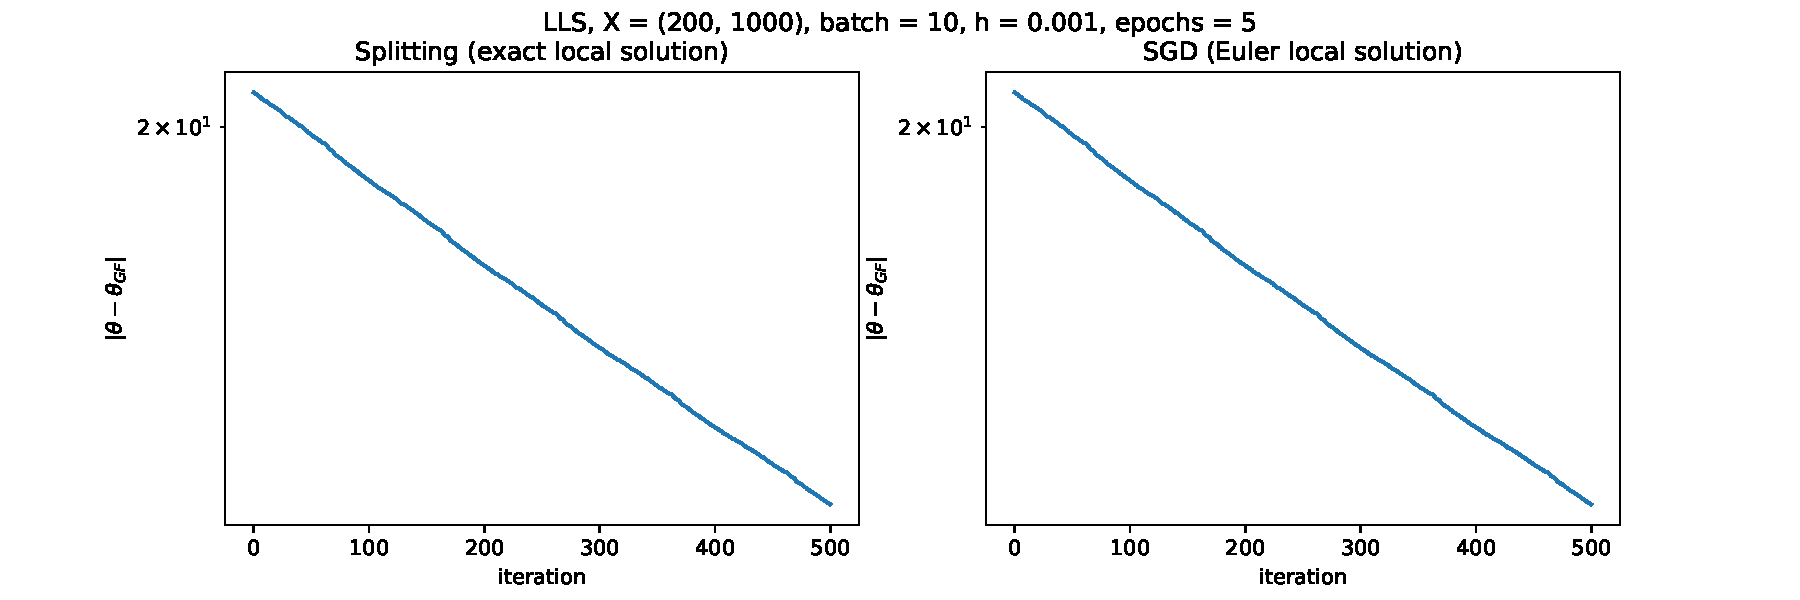
\includegraphics[width=0.85\textwidth]{{robustness_to_stepsize/sgd_split0.001}.pdf} \\
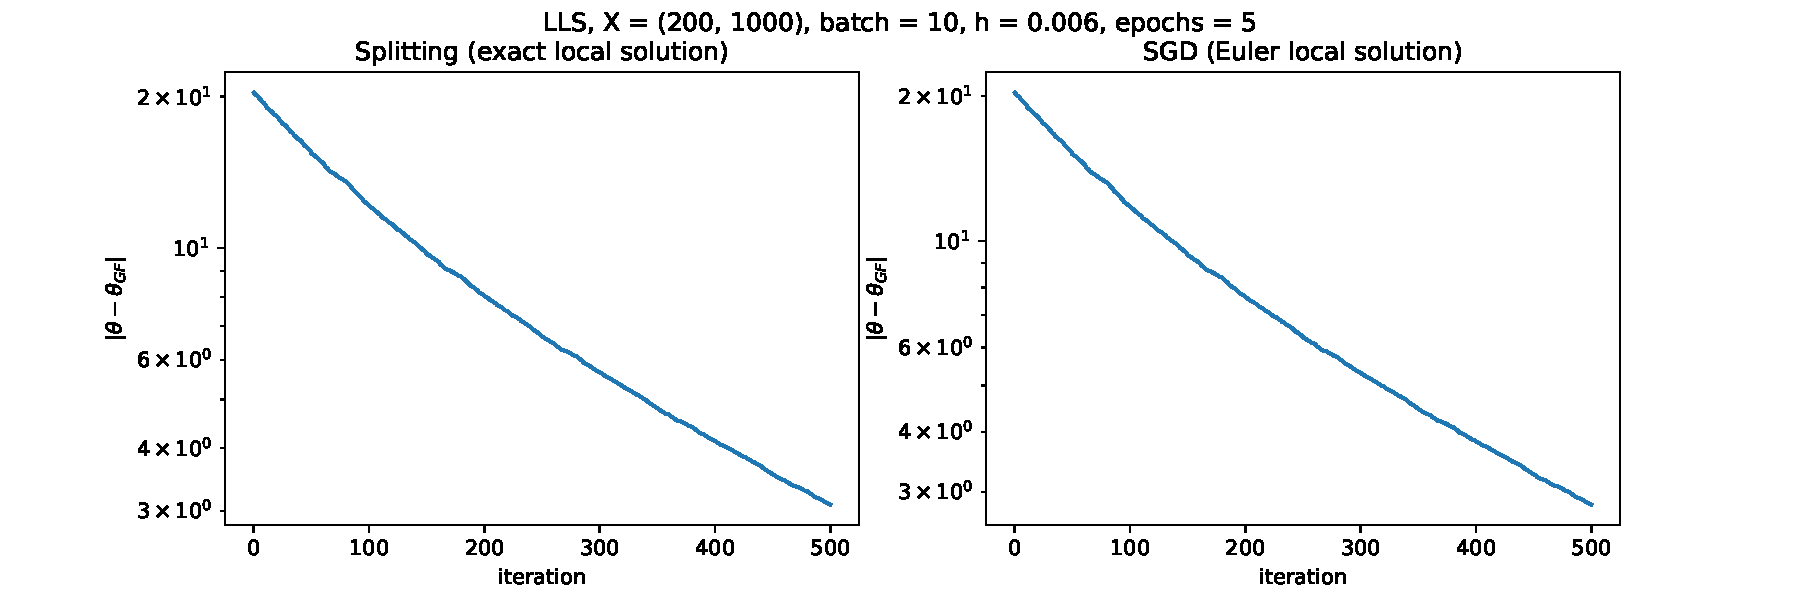
\includegraphics[width=0.85\textwidth]{{robustness_to_stepsize/sgd_split0.006}.pdf} \\
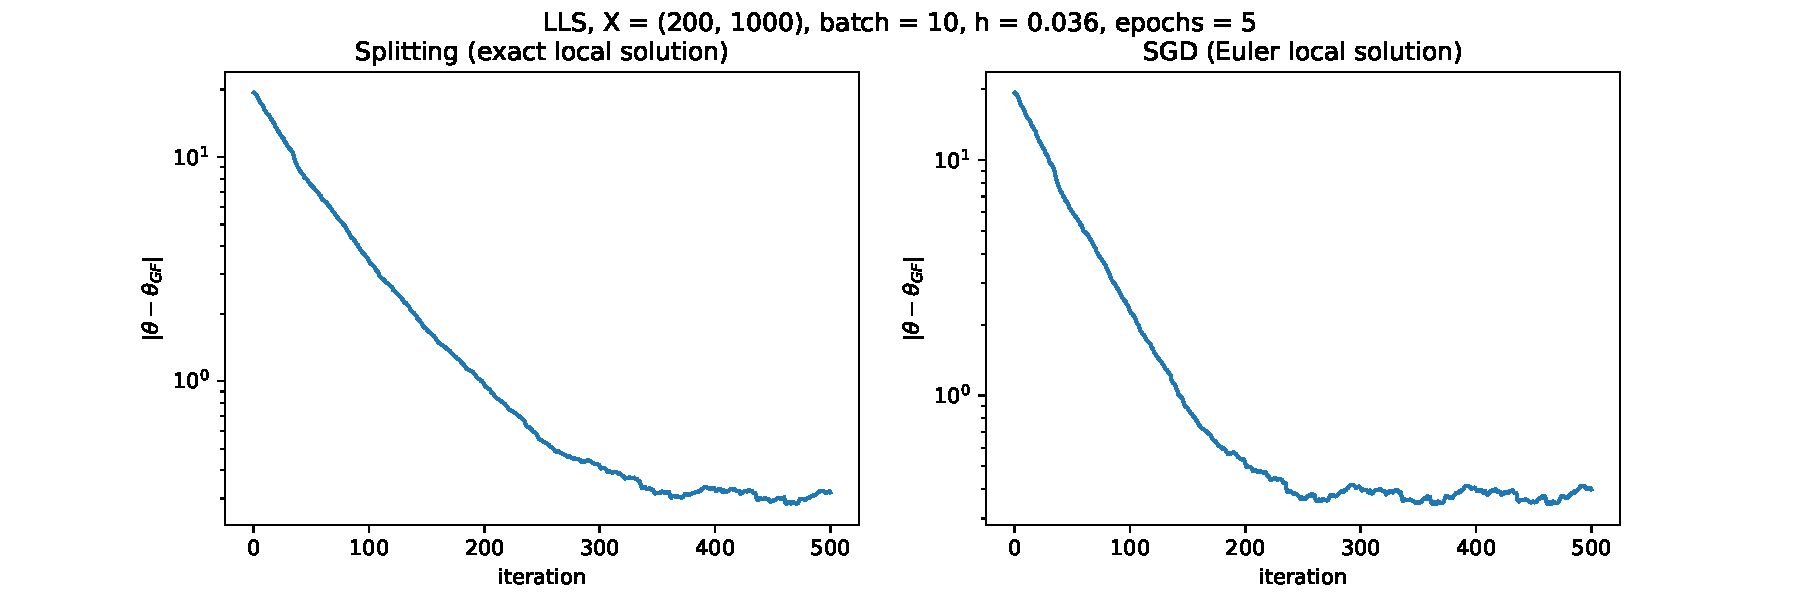
\includegraphics[width=0.85\textwidth]{{robustness_to_stepsize/sgd_split0.036}.pdf} \\
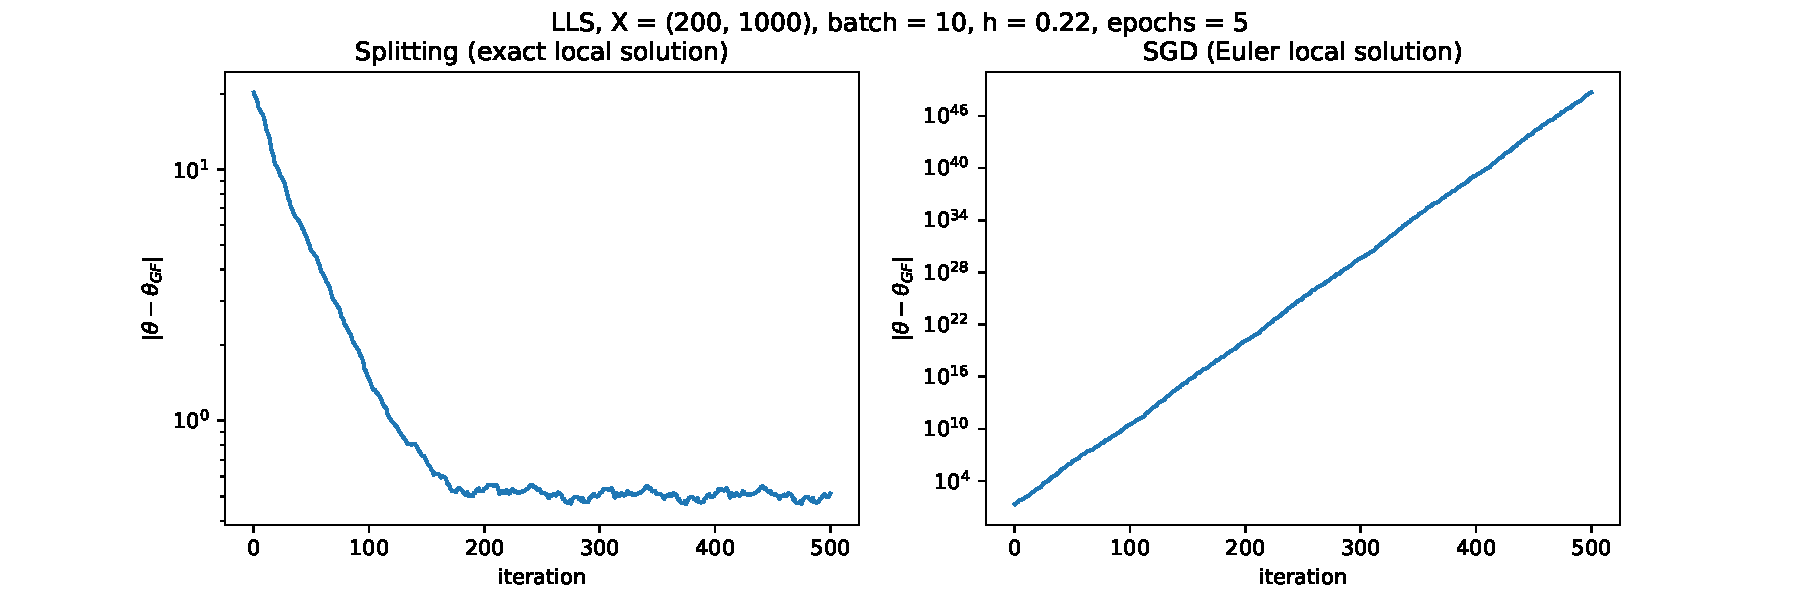
\includegraphics[width=0.85\textwidth]{{robustness_to_stepsize/sgd_split0.22}.pdf} \\
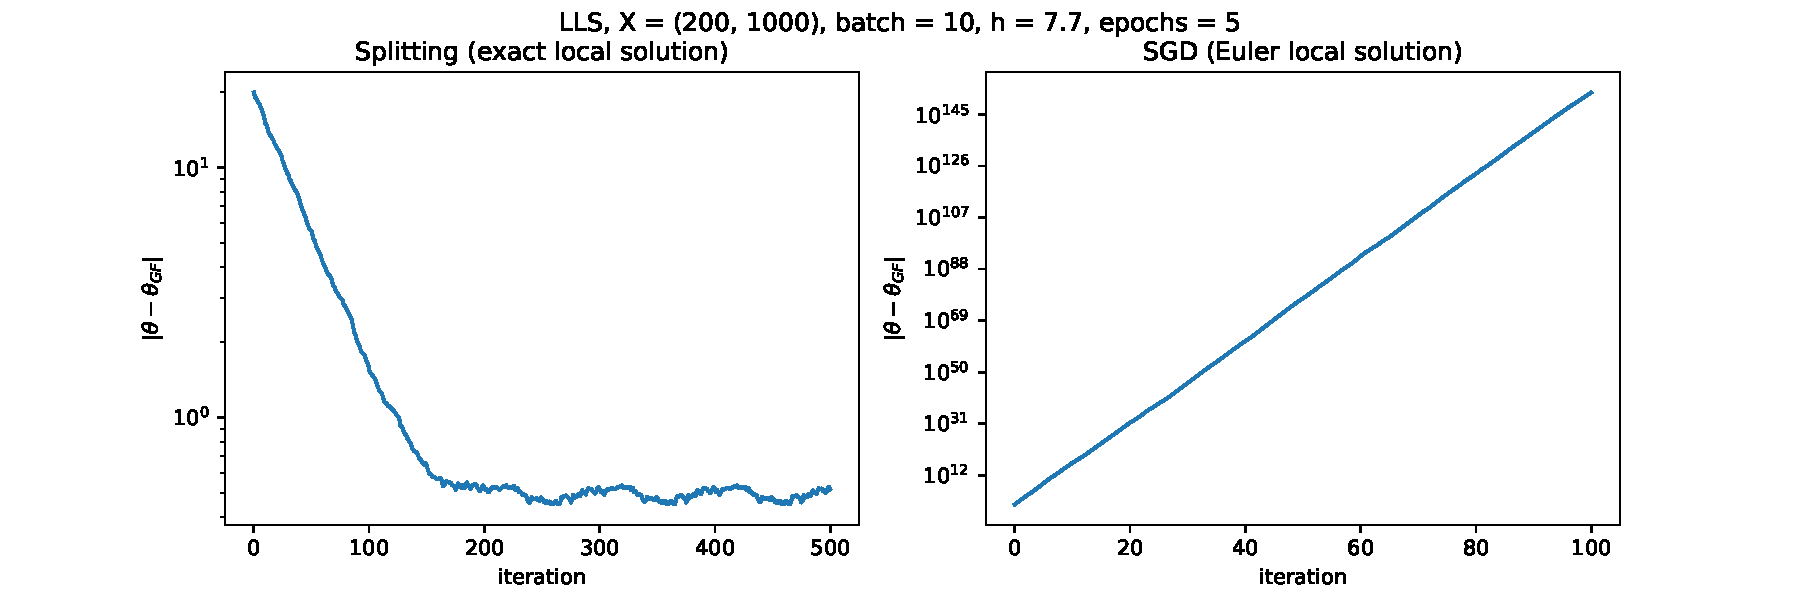
\includegraphics[width=0.85\textwidth]{{robustness_to_stepsize/sgd_split7.7}.pdf} \\
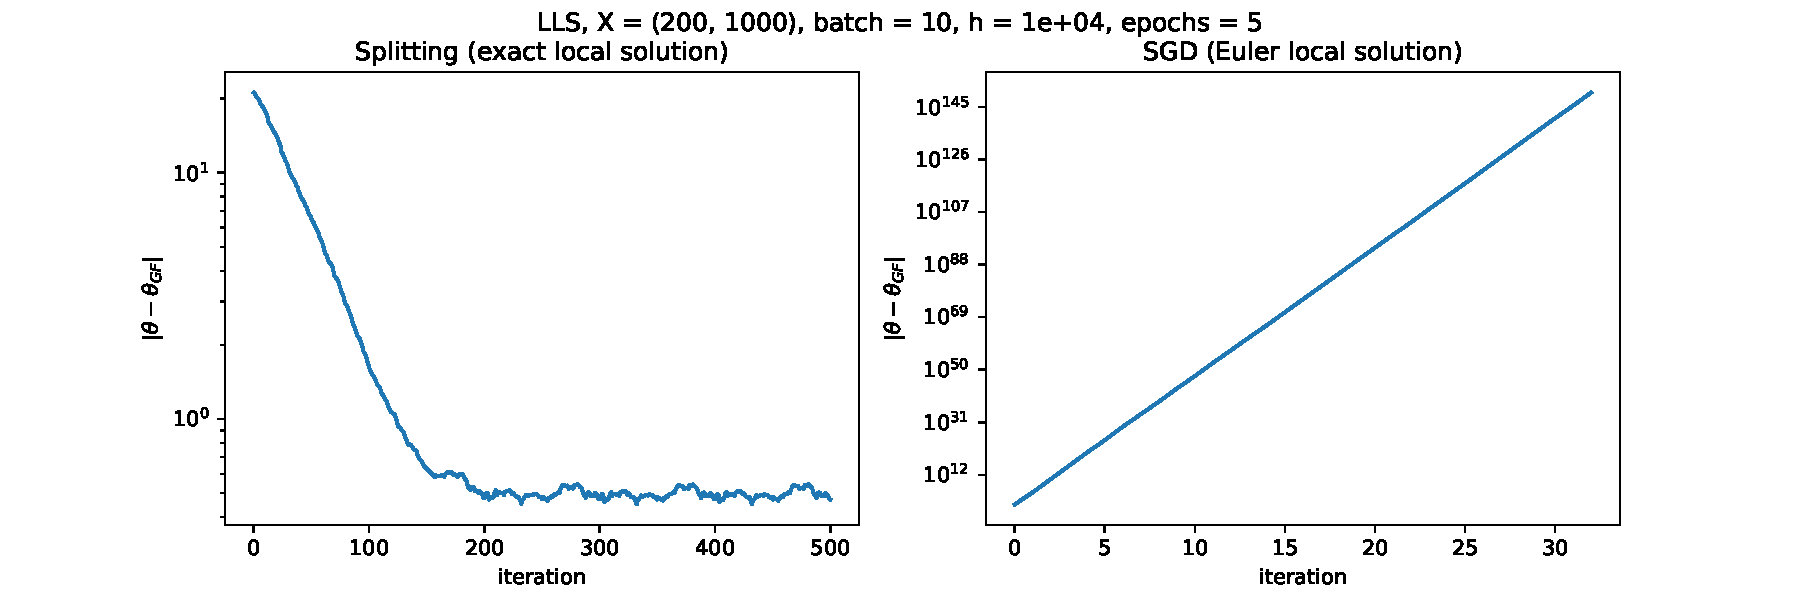
\includegraphics[width=0.85\textwidth]{{robustness_to_stepsize/sgd_split1e+04}.pdf}
\caption{Linear Least Squares, $X \in \mathbb{R}^{200 \times 1000}, b = 10$}
\end{figure}


\begin{figure}
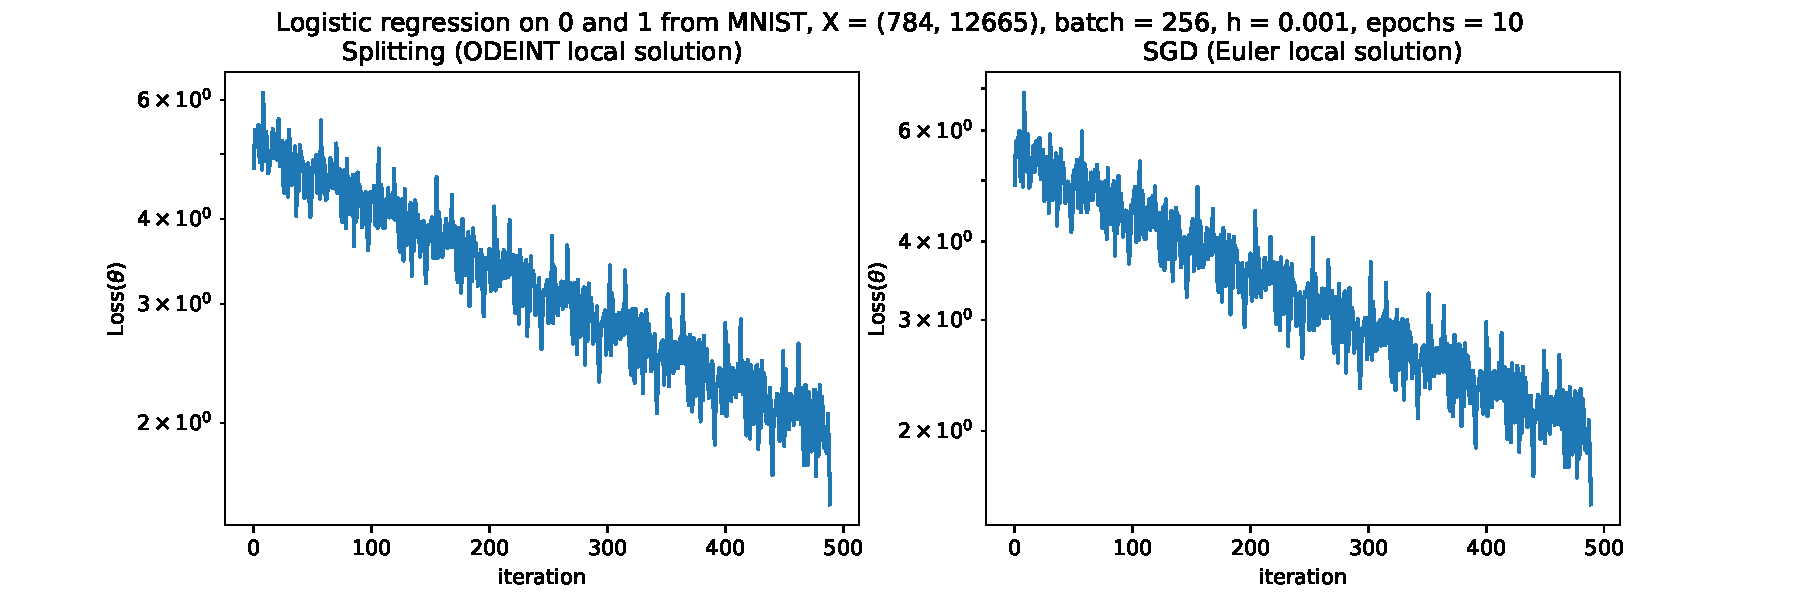
\includegraphics[width=0.85\textwidth]{{robustness_to_stepsize/sgd_split_logreg0.001}.pdf} \\
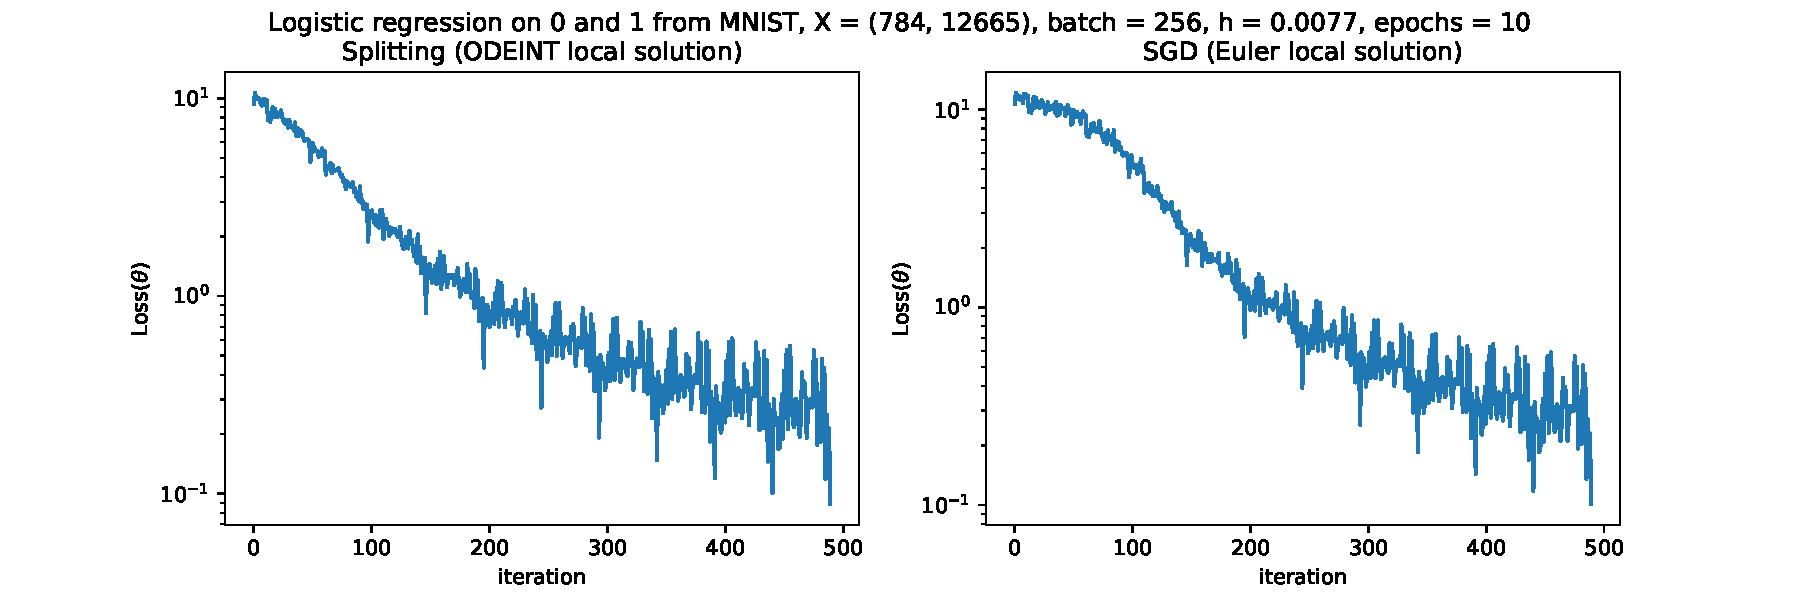
\includegraphics[width=0.85\textwidth]{{robustness_to_stepsize/sgd_split_logreg0.0077}.pdf} \\
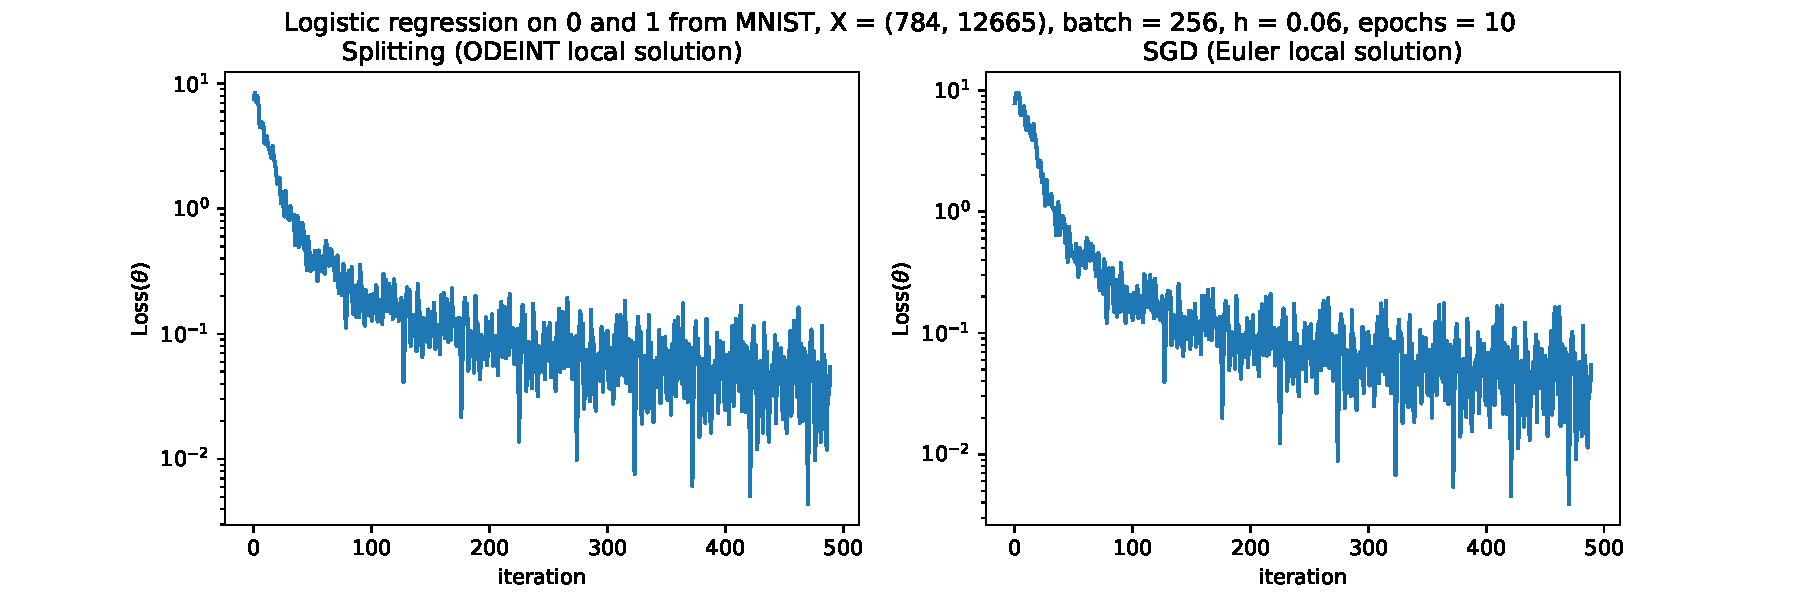
\includegraphics[width=0.85\textwidth]{{robustness_to_stepsize/sgd_split_logreg0.06}.pdf} \\
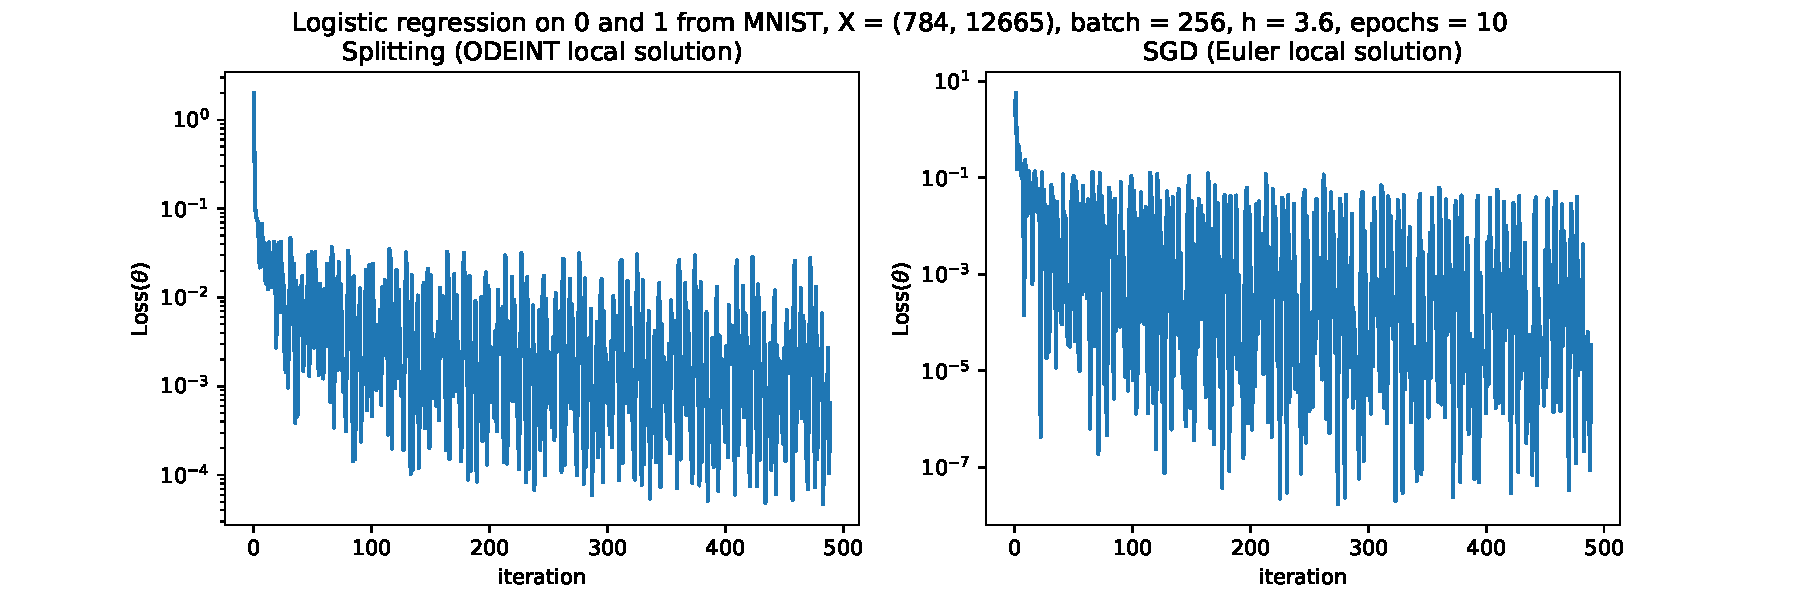
\includegraphics[width=0.85\textwidth]{{robustness_to_stepsize/sgd_split_logreg3.6}.pdf} \\
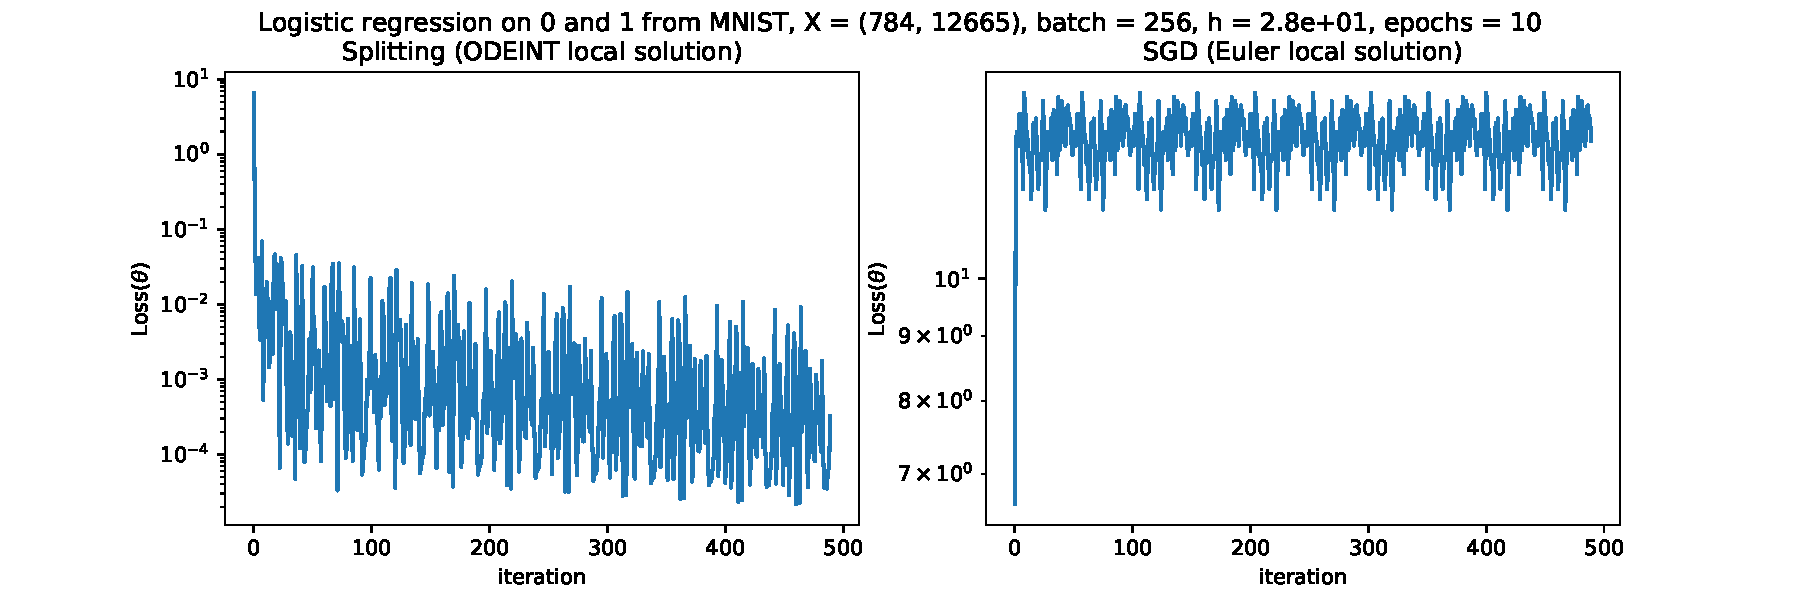
\includegraphics[width=0.85\textwidth]{{robustness_to_stepsize/sgd_split_logreg2.8e+01}.pdf} \\
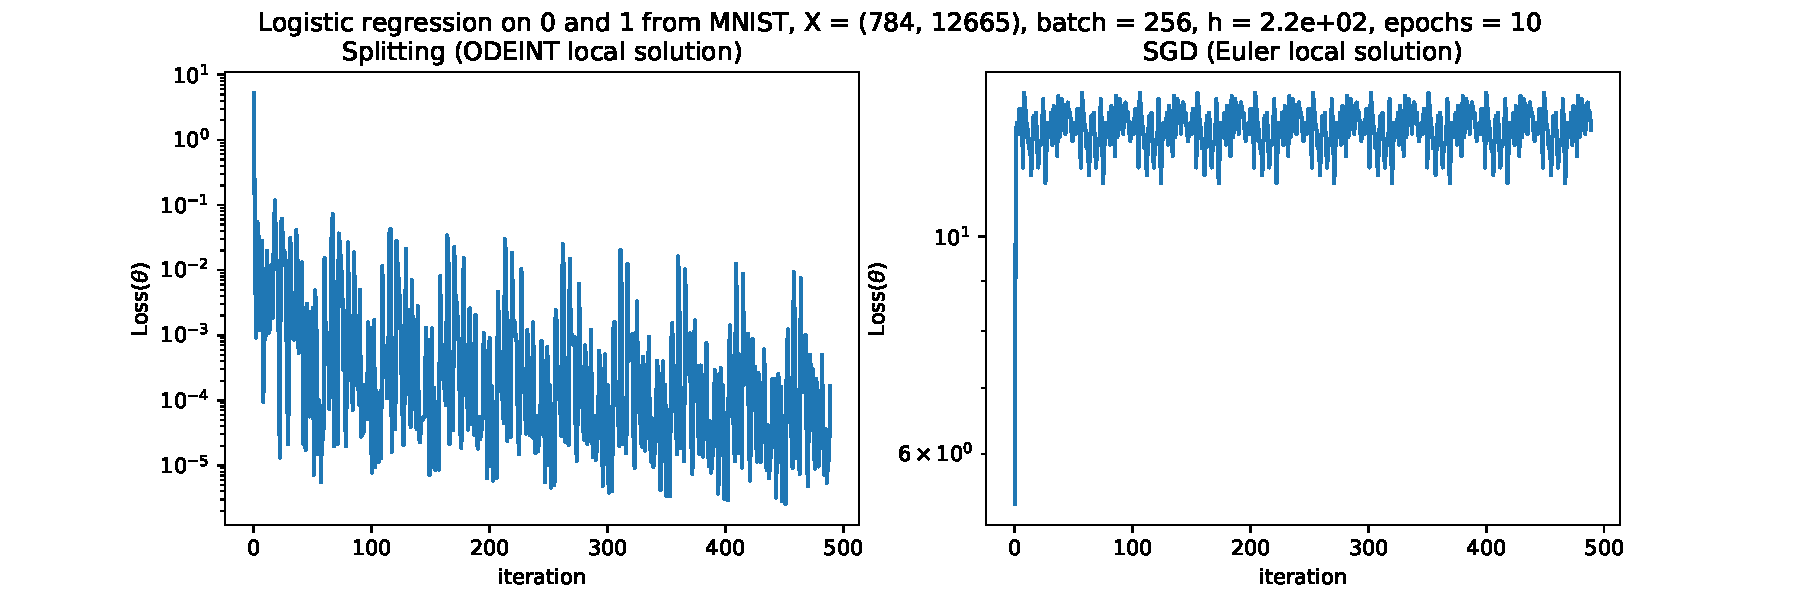
\includegraphics[width=0.85\textwidth]{{robustness_to_stepsize/sgd_split_logreg2.2e+02}.pdf}
\caption{Binary logistic regression on 0 and 1 from MNIST dataset}
\end{figure}

\begin{figure}
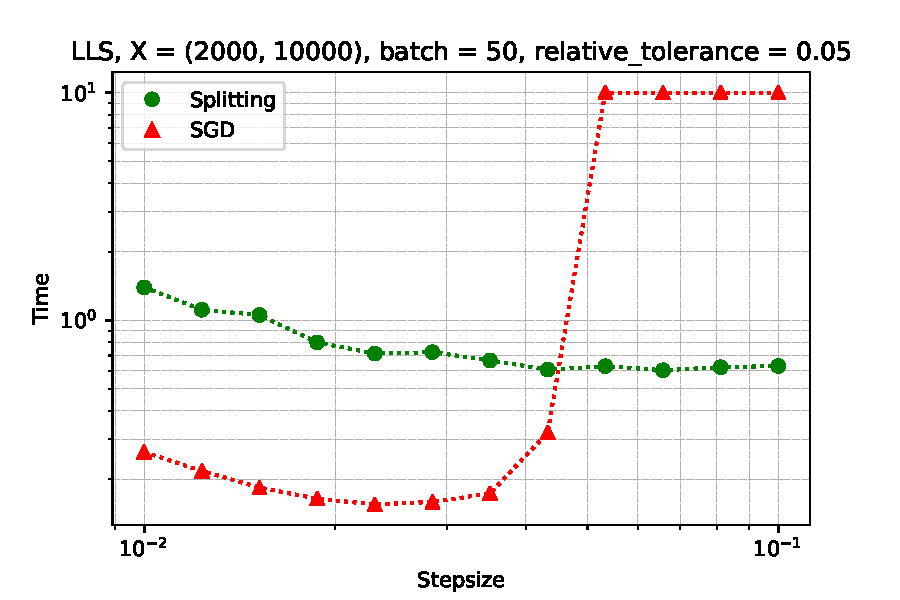
\includegraphics[width=0.85\textwidth]{sgd_split_iterations_lls.pdf} \\
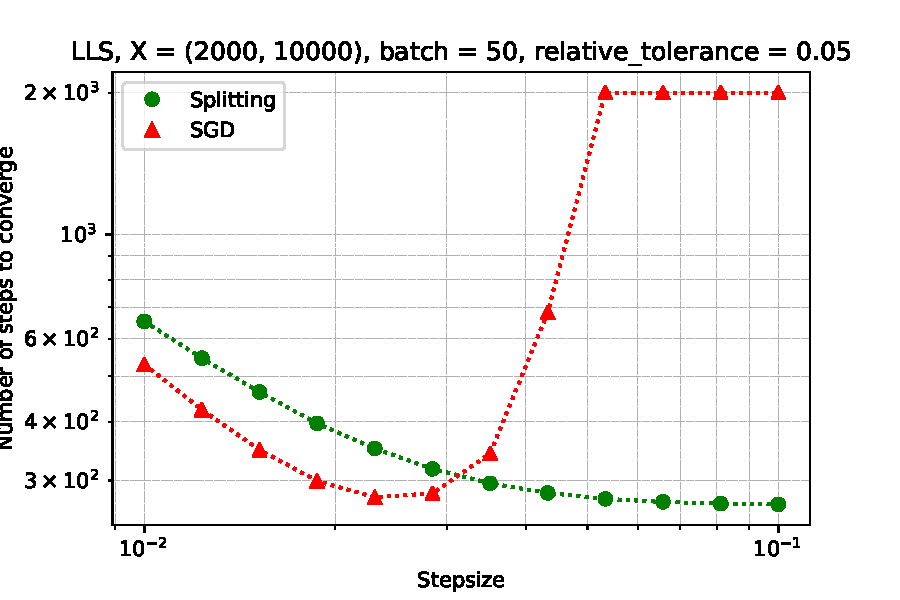
\includegraphics[width=0.85\textwidth]{sgd_split_time_lls.pdf}

\caption{Random linear system. Averaging on 30 runs}
\end{figure}

\begin{figure}
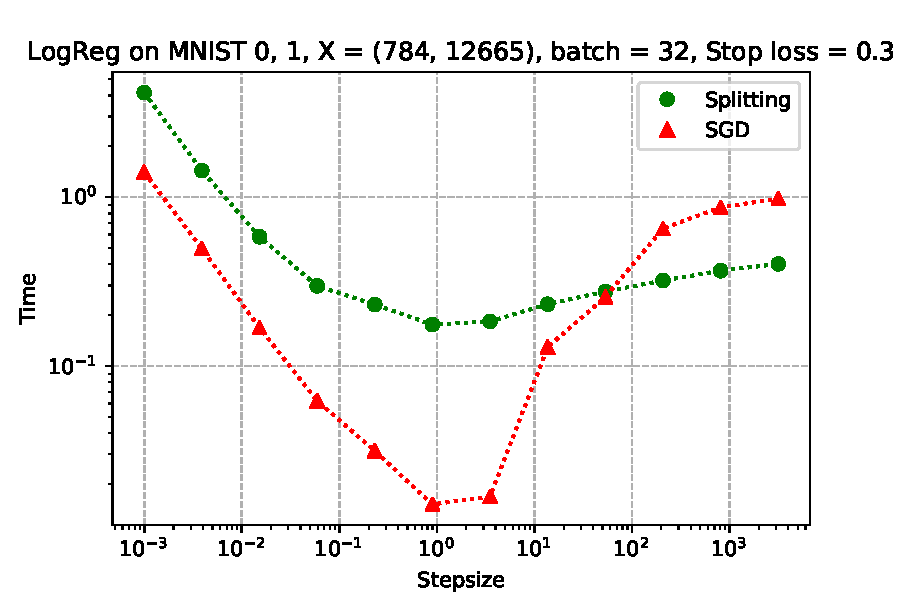
\includegraphics[width=0.85\textwidth]{sgd_split_iterations_logreg.pdf} \\
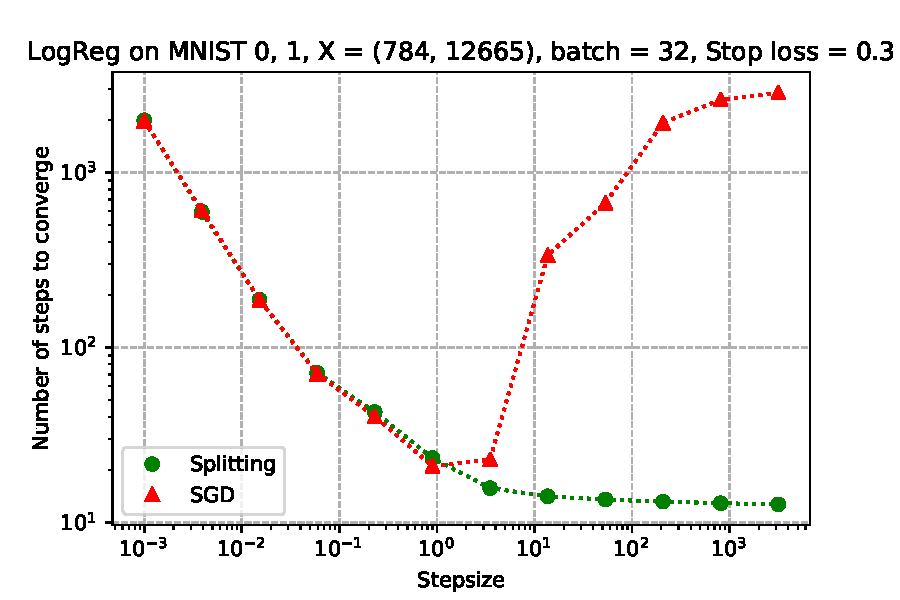
\includegraphics[width=0.85\textwidth]{sgd_split_time_logreg.pdf}

\caption{MNIST 0,1. Binary logistic regression. Averaging on 30 runs}
\end{figure}

\newpage

\bibliography{biblio}
\bibliographystyle{iclr2019_conference}

\end{document}